\subsection{Kavrayskiy 7 Projektion}
\label{sec:kravrayskiy}
Die Kavrayskiy 7 Projektion ist der Robinson Projektion sehr ähnlich. Sie stellt die Erde wieder annähernd oval dar. Die Breitenkreise werden in dieser Projektion als Geraden dargestellt. Diese Projektion stellt einen Kompromiss zwischen winkeltreuen und flächentreuen Projektionen dar. Die Pole sind in dieser Darstellung sehr breit gezogen. \\
Formel:\\
\begin{eqnarray*}
\mathcal {X} & = & \dfrac {3\lambda } {2\pi \sqrt {\dfrac {\pi ^2}{3}-\varphi ^2}}\\
\mathcal {Y} & = &\varphi
\end{eqnarray*}\\

\begin{figure}[hbtp]
\centering
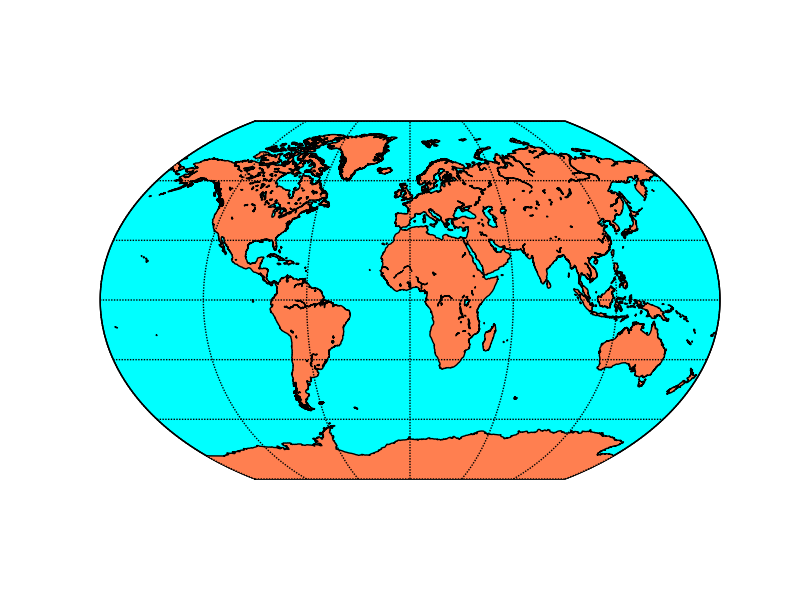
\includegraphics[scale=0.5,origin=c]{/Users/student/seminar/Kartendarstellungen/seminar/kav7} \caption{Kavarayskiy 7 Projektion}
\end{figure}
\newpage 